\documentclass{article}
\usepackage[final]{neurips_2020}
\usepackage[utf8]{inputenc}
\usepackage{ctex}
\usepackage[T1]{fontenc}
\usepackage{hyperref}
\usepackage{url}
\usepackage{booktabs}
\usepackage{algorithm}
\usepackage{algpseudocode}  % 这个包用于算法伪代码

\usepackage{amsfonts}
\usepackage{amsmath}
\usepackage{nicefrac}
\usepackage{microtype}
\usepackage{indentfirst}
\usepackage{listings}
\usepackage{graphicx}
\usepackage{float}

\usepackage[dvipsnames]{xcolor}
\lstset{
    language=Python,
    basicstyle=\ttfamily,
    breaklines=true,
    keywordstyle=\bfseries\color{NavyBlue},
    morekeywords={},
    emph={self},
    emphstyle=\bfseries\color{Rhodamine},
    commentstyle=\itshape\color{black!50!white},
    stringstyle=\bfseries\color{PineGreen!90!black},
    columns=flexible,
    numbers=left,
    numbersep=2em,
    numberstyle=\footnotesize,
    frame=single,
    framesep=1em,
    showstringspaces=false
}
\setlength{\parindent}{2em}

\title{中山大学计算机院本科生实验报告\\
    (2024学年秋季学期)}

\begin{document}
\maketitle
课程名称:强化学习与博弈论 \qquad\qquad\qquad\qquad\qquad\qquad
批改人:
\begin{table*}[h]
    \centering
    \begin{tabular}{|c|c|c|c|} \hline
        实验    & Assignment1                 & 专业(方向) & 计算机科学与技术 计科一班 \\ \hline
        学号    & 21307099                           & 姓名     & 李英骏           \\\hline
        Email & \texttt{liyj323@mail2.sysu.edu.cn} & 完成日期   & \today        \\\hline
    \end{tabular}
\end{table*}
\tableofcontents

\newpage
\section{实验背景}
Cliff Walk 是强化学习中的经典环境,用于测试算法在高风险场景下的表现。该环境由一个 $4 \times 12$ 的网格组成,起点 $S$ 位于左下角,终点 $G$ 位于右下角。起点和终点之间的悬崖区域会导致代理掉入后受到 $-100$ 的惩罚,并返回到起点。每一步移动都会收到 $-1$ 的奖励。

在该实验中,我们分别使用 SARSA 和 Q-learning 算法训练代理学习最优路径,并对比两种算法在路径选择和奖励表现上的差异。

\section{算法核心思路}
SARSA 和 Q-learning 都是基于 Q-learning 的值迭代算法。其核心在于通过更新 Q 值来指导代理选择动作。具体可见代码中的注释,如下:

\subsection{SARSA 算法}
SARSA 算法的更新公式如下:
\[
Q(S, A) \gets Q(S, A) + \alpha \cdot \left[ R + \gamma \cdot Q(S', A') - Q(S, A) \right]
\]
其中:
\begin{itemize}
    \item $S, A$:当前状态和动作;
    \item $R$:即时奖励;
    \item $S', A'$:下一状态和实际选择的动作;
    \item $\alpha$:学习率;
    \item $\gamma$:折扣因子。
\end{itemize}

\subsection{Q-learning 算法}
Q-learning 算法的更新公式如下:
\[
Q(S, A) \gets Q(S, A) + \alpha \cdot \left[ R + \gamma \cdot \max_a Q(S', a) - Q(S, A) \right]
\]
其中:
\begin{itemize}
    \item $S, A$:当前状态和动作;
    \item $R$:即时奖励;
    \item $S'$:下一状态;
    \item $\max_a Q(S', a)$:下一状态下的最大 Q 值;
    \item $\alpha$:学习率;
    \item $\gamma$:折扣因子。
\end{itemize}

\section{实验设计}
\subsection{实验环境}
实验环境为 Cliff Walk,网格大小为 $4 \times 12$,起点和终点分别位于左下角和右下角。悬崖区域位于底部。

\subsection{实验参数}
实验参数设置如下:
\begin{itemize}
    \item 学习率 $\alpha = 0.5$;
    \item 折扣因子 $\gamma = 0.9$;
    \item 探索率 $\epsilon = 0.1$;
    \item 最大训练回合数:5000。
\end{itemize}

\subsection{实验目标}
通过 SARSA 和 Q-learning 算法训练代理,比较以下两点:
\begin{enumerate}
    \item 两种算法生成的行走路径;
    \item 两种算法的奖励曲线变化趋势。
\end{enumerate}

\section{实验结果与分析}
\subsection{SARSA 算法路径}
SARSA 算法的路径如图 \ref{fig:sarsa_path} 所示。

\begin{figure}[h!]
    \centering
    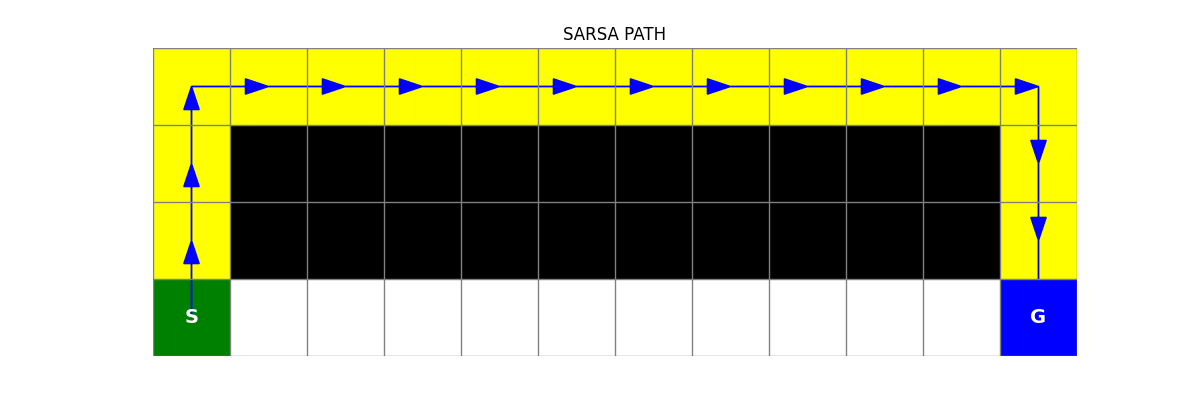
\includegraphics[width=0.9\textwidth]{sarsa_path.png}
    \caption{SARSA 算法路径}
    \label{fig:sarsa_path}
\end{figure}

SARSA 算法的路径明显避开了悬崖区域,选择了更保守的路线。agnet通过顶部区域向右移动,再从顶部到终点。路径表明 SARSA 倾向于学习更安全的策略。

\subsection{Q-learning 算法路径}
Q-learning 算法的路径如图 \ref{fig:qlearning_path} 所示。

\begin{figure}[h!]
    \centering
    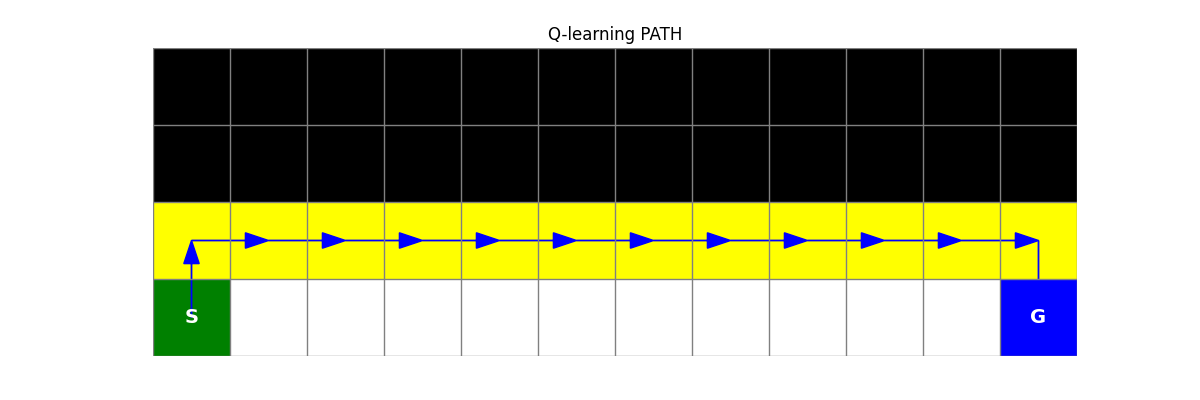
\includegraphics[width=0.9\textwidth]{qlearning_path.png}
    \caption{Q-learning 算法路径}
    \label{fig:qlearning_path}
\end{figure}

Q-learning 算法中agent直接沿着悬崖上方移动,选择了一条更短的路径到达终点。这表明 Q-learning 倾向于冒险以追求最优路径。

\subsection{奖励曲线分析}
每回合的总奖励变化如图 \ref{fig:reward_curve} 所示,下面那张图 \ref{fig:reward_curve_smoothed} 是平滑后的。

\begin{figure}[h!]
    \centering
    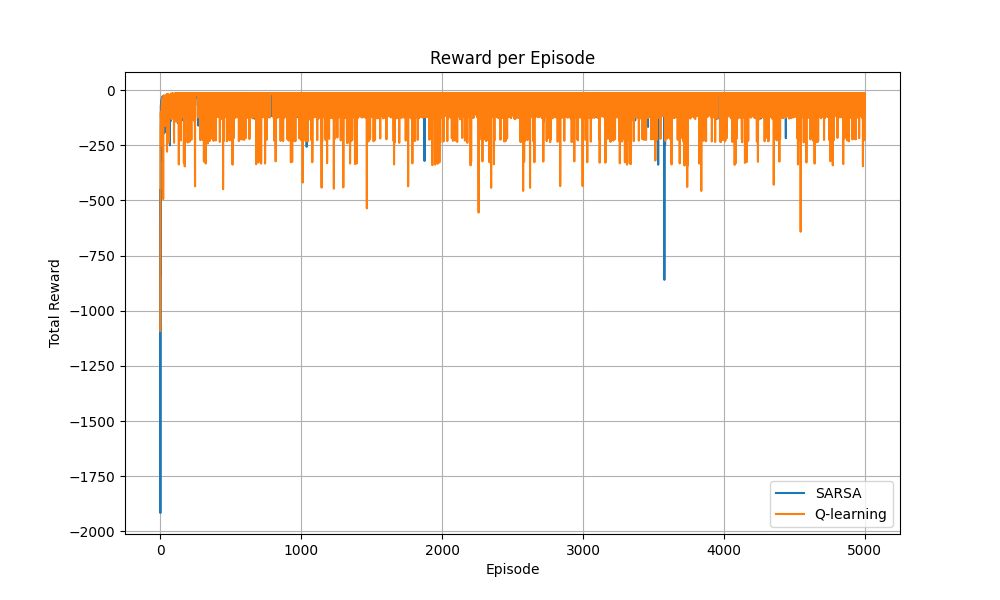
\includegraphics[width=0.9\textwidth]{reward_curve.png}
    \caption{每回合奖励曲线}
    \label{fig:reward_curve}
\end{figure}
\begin{figure}[H]
    \centering
    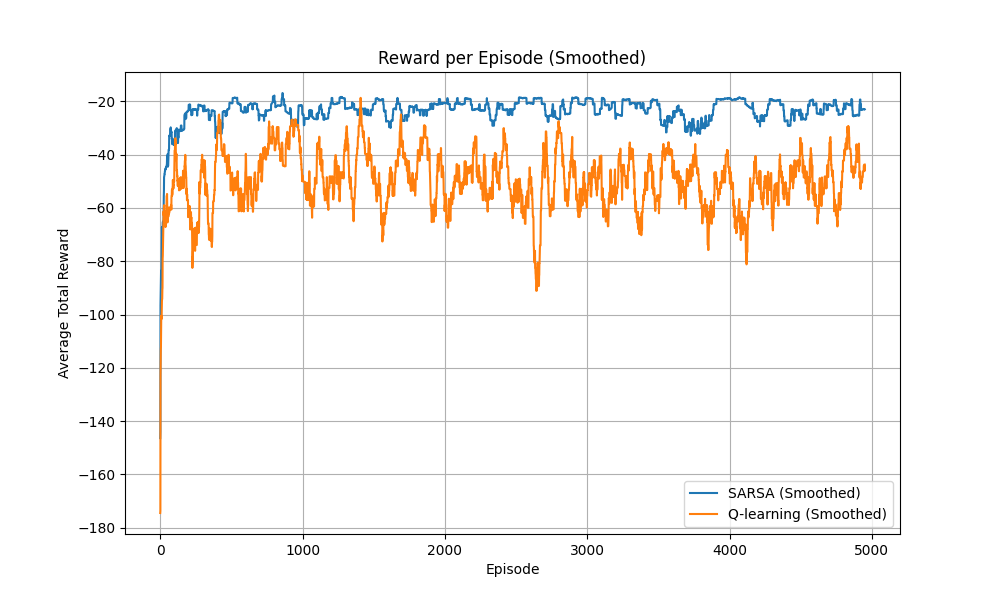
\includegraphics[width=0.9\textwidth]{reward_curve_smoothed.png}
    \caption{每回合奖励曲线(smoothed)}
    \label{fig:reward_curve_smoothed}
\end{figure}

从奖励曲线可以看出:
\begin{itemize}
    \item SARSA 的奖励曲线收敛更快,波动较小。
    \item Q-learning 的奖励曲线初始阶段波动较大,最终逐渐收敛,但仍有较大的波动。
\end{itemize}

\section{结论}
通过实验结果分析,我们可以得出以下结论:
\begin{itemize}
    \item SARSA 更适合高风险场景,其更新基于当前策略,倾向于学习保守路径。
    \item Q-learning 更适合追求全局最优解的场景,其更新基于最优动作值,但可能带来更高的风险。
\end{itemize}

\section*{参考}
\begin{enumerate}
    \item OpenAI Gym Documentation: \texttt{https://www.gymlibrary.dev/}
\end{enumerate}

\end{document}
